\documentclass[10pt]{article}

\usepackage[T1]{fontenc}
\usepackage[left=0.82in,right=0.82in,top=0.70in,bottom=0.70in]{geometry}
\usepackage{amsmath,amssymb,mathtools}
\usepackage{booktabs,tabularx,array}
\usepackage{enumitem}
\usepackage{graphicx}
\usepackage{placeins}
\usepackage{xcolor}
\usepackage{hyperref}
\usepackage{microtype}

\hypersetup{
  colorlinks=true,
  linkcolor=blue!45!black,
  citecolor=blue!45!black,
  urlcolor=blue!45!black
}

\setlength{\emergencystretch}{3em}
\setlist[enumerate]{topsep=3pt,itemsep=2pt,leftmargin=1.6em}
\setlist[itemize]{topsep=3pt,itemsep=2pt,leftmargin=1.5em}
\newcommand{\Gref}{G_{\mathrm{ref}}}
\newcommand{\Gint}{G_{\mathrm{int}}}
\newcommand{\dd}{\,\mathrm d}

\title{Paper Corpus Generation:\\
An End-to-End Account}
\author{}
\date{27 July 2026}

\begin{document}
\maketitle

\begin{abstract}
This note follows one case from a random seed to the arrays read by the
trainer.  The replacement corpus contains four kinds of periodic water-wave
states: Stokes waves, Tanaka-profile sums, Benjamin--Feir perturbations, and
JONSWAP/TMA random seas.  Every label is computed with the same fixed
discrete Dirichlet--Neumann operator.

A draw must first lie in the stated parameter range of its family.  A
time-dependent draw is then retained only if one fixed-step calculation both
returns a complete finite trajectory and keeps the free surface above the
bottom.  No rule based on visual roughness, sign changes, slope, Hamiltonian
drift, or model error removes a case.  This document is the specification of
the replacement corpus; the corpus itself has not yet been generated.
\end{abstract}

\section{Objects and guiding rules}

The horizontal interval is $0\leq x<L$, with periodic endpoints and
$L=2\pi$, and gravity is set to one.  A \emph{case} is one sampled initial
surface elevation $\eta_0(x)$, one sampled value $\xi_0(x)$ of the velocity
potential at the surface, and one fixed water depth $h>0$.  A
\emph{trajectory} is the computed evolution of that case.  A \emph{row} is
one retained time from an accepted case.

The case, rather than the row, is the unit of splitting, rejection, and
training weight.  This matters because an accepted Stokes case stores one
row, whereas accepted Tanaka and Benjamin--Feir cases each store 200 rows.
Counting all stored rows equally would therefore give a long trajectory much
more influence than a static wave.

The construction follows four elementary rules.
\begin{enumerate}
  \item Fix the numerical meaning of a label before sampling any cases.
  \item Assign a case to training, validation, or test before seeing whether
        its numerical calculation succeeds.
  \item Replace a failed attempt only within its original parameter category.
  \item Select stored times only after the entire case has been accepted.
\end{enumerate}

\section{The common numerical label}
\label{sec:target}

For given $\eta$, $\xi$, and $h$, let $\varphi(x,y)$ solve
\begin{equation}
  \varphi_{xx}+\varphi_{yy}=0,\qquad
  \varphi_y(x,-h)=0,\qquad
  \varphi(x,\eta(x))=\xi(x).
\end{equation}
Subscripts denote partial derivatives.
The physical Dirichlet--Neumann operator is
\begin{equation}
  G(\eta;h)\xi
  =\left(\varphi_y-\eta_x\varphi_x\right)_{y=\eta(x)}.
  \label{eq:physical-dno}
\end{equation}
It is the slope-corrected upward derivative of the solution $\varphi$ at the
free surface.  In the Zakharov equations it is also $\eta_t$, the
instantaneous rate of change of the surface.

The dataset does not claim to evaluate \eqref{eq:physical-dno} exactly.
Instead, it freezes one discrete reference calculation.  All fields use
$N=1024$ equally spaced points
$x_\ell=2\pi\ell/1024$, $\ell=0,\ldots,1023$.  Since the period is $2\pi$,
the Fourier wavenumbers are the integers.  Let $P_{128}$ discard all modes with
$|k|>128$, and let $P_{128}^{\circ}$ additionally remove the spatial mean.
Let $\mathcal G_{6}^{1024,8}$ denote the implemented order-six
Craig--Sulem calculation on 1024 points with padding factor eight.  The label
is
\begin{equation}
  \boxed{
  \Gref(\eta;h)\xi
  =
  P_{128}^{\circ}\!\left[
    \mathcal G_{6}^{1024,8}
      (P_{128}\eta;h)(P_{128}\xi)
  \right].}
  \label{eq:reference-target}
\end{equation}
The calculation is performed in 64-bit arithmetic.  Only the final spatial
arrays are converted to 32-bit form for storage.  Thus every retained row is
\begin{equation}
  \left(
    P_{128}\eta(t),\
    P_{128}\xi(t),\
    h,\
    t,\
    \Gref(\eta(t);h)\xi(t)
  \right).
  \label{eq:stored-row}
\end{equation}
The model is trained to reproduce the fixed discrete quantity in
\eqref{eq:reference-target}.  Approximation of the continuum operator
\eqref{eq:physical-dno} is a separate question requiring convergence tests
in truncation order, grid size, and padding.
Every constructor removes the spatial mean of $\xi$; this fixes the
irrelevant freedom to add a constant to the potential.

\section{One case from beginning to end}
\label{sec:pipeline}

The complete production path is:
\begin{enumerate}
  \item Assign a family, parameter category, data split, and deterministic
        random-number key, then draw and record all initial-condition
        parameters.
  \item Check the family's stated parameter rules and construct
        $(\eta_0,\xi_0,h)$.  Before rollout, the assembled initial arrays
        must be finite, \(h>0\), and \(h+\eta_0>0\) on the grid.
  \item For a Stokes case, evaluate \eqref{eq:reference-target} at $t=0$.
        For the other families, run the single fixed-step calculation in
        Section~\ref{sec:rollout}.
  \item Apply the whole-case decision in Section~\ref{sec:rollout}.  A failed
        trajectory contributes no rows, including no apparently good prefix.
  \item After acceptance, choose the retained times and write their arrays,
        numerical diagnostics, and checksum.
  \item Count an accepted case toward its original parameter category.  If it
        failed, draw a new case in that same category.
  \item When every family and split quota is complete, build a checked index
        into the array files and pass that index to the trainer.
\end{enumerate}
The sampled specification is written before numerical work, so an
interrupted case can be replayed without drawing a replacement.  An
unexpected construction error, including failure of the initial-array
conditions above, stops the run; it is not silently relabeled as an ordinary
rejected draw.  Checksums detect missing or changed array files.

\section{How the four initial-condition families are sampled}
\label{sec:families}

A \emph{parameter category} is a pre-set part of one family's parameter
range that receives its own accepted-case count.  The categories keep important
regimes from disappearing by chance.  Uniform sampling on $[a,b]$ means
that every interval of the same length is equally likely.  Log-uniform
sampling means that $\log h$ is uniform.  A uniform simplex split of a
positive number $A$ chooses nonnegative weights $w_j$ with
$\sum_jw_j=1$ and sets the pieces to $Aw_j$.

\begin{table}[ht]
  \centering
  \small
  \caption{The four training families.  A horizon is needed only for a
  time-dependent family.}
  \label{tab:families}
  \begin{tabularx}{\textwidth}{
    @{}>{\raggedright\arraybackslash}p{0.17\textwidth}
       >{\raggedright\arraybackslash}p{0.13\textwidth}
       >{\raggedright\arraybackslash}X
       >{\raggedright\arraybackslash}p{0.15\textwidth}@{}}
    \toprule
    Family & Categories & Main distinction & Horizon / retained rows \\
    \midrule
    Stokes
      & 4
      & finite/deep branch and low/moderate steepness
      & static / 1 \\
    Tanaka
      & 11
      & regime, number of crests, and number moving right
      & $T=200$ / 200 \\
    Benjamin--Feir
      & 66
      & one feasible carrier--sideband integer pair per category
      & $T=200$ / 200 \\
    JONSWAP/TMA
      & 27
      & shallow/finite/deep, peak enhancement, and direction balance
      & last $0.08$-grid time not exceeding 16 peak periods / 16 \\
    \bottomrule
  \end{tabularx}
\end{table}

\subsection{Fifth-order Stokes states}

A Stokes draw first fixes one of four parameter categories:
\[
  \{\text{finite},\text{deep}\}
  \times
  \{0.005\leq ka<0.03,\quad 0.03\leq ka\leq0.15\}.
\]
Here $k$ is the carrier wavenumber and $a$ is the expansion-amplitude
parameter of the fifth-order formula.  Because the first harmonic receives
nonlinear corrections, $a$ is not exactly the realized first-harmonic
amplitude.  The common parameter interval is
\[
  0.000766\leq a\leq0.011494.
\]
For the finite-depth branch, the mode number is
$n\in\{14,\ldots,26\}$, the wavenumber is $k=n$, and
\[
  0.02\leq h\leq1.5,\qquad 0.5\leq kh\leq5.
\]
For the deep branch,
\[
  n\in\{1,\ldots,20\},\qquad 4\leq h\leq50,\qquad kh\geq5.
\]
The program lists the modes compatible with the chosen category and selects one
uniformly.  It then draws $h$ log-uniformly in the compatible depth interval,
draws a phase $\phi$ uniformly on $[0,2\pi)$, and draws $a$ uniformly from the
intersection of the common amplitude interval and the chosen $ka$ interval.
The code evaluates Fenton's fifth-order analytic Stokes expansion, using its
finite-depth coefficients or deep-water limit, to construct
$(\eta_0,\xi_0)$~\cite{fenton1985}.  The parameter ranges, four parameter
categories, random phase, and depth law above are corpus choices rather than
claims made by Fenton.

The finite-depth formula is used only in its intended Stokes regime.  For
phase $\theta=kx+\phi$, write its elevation as
\[
  \eta_5(\theta)=\sum_{r=1}^{5}E_r\cos(r\theta),
\]
where $E_r$ is the coefficient of harmonic $r$.  Let $H_{4096}$ be the
largest sampled value of $\eta_5$ minus its smallest sampled value on 4096
equally spaced phases, and define
\[
  H_+
  =
  H_{4096}
  +\frac14\left(\frac{2\pi}{4096}\right)^2
    \sum_{r=1}^{5}r^2|E_r|.
\]
The last term bounds the possible height missed between two phase samples.
With wavelength $\lambda=2\pi/k$, the required support condition is
\begin{equation}
  \mathrm{Ur}_+
  =\frac{H_+\lambda^2}{h^3}
  \leq26.
  \label{eq:ursell}
\end{equation}
This is a conservative Ursell-number restriction for the fifth-order
formula, not a fitted predictor of whether a numerical rollout would
survive~\cite{fenton1985,zhao2024}.  If \eqref{eq:ursell} fails, the mode,
depth, phase, and parameter category remain fixed and only the amplitude is
redrawn, with at most 1000 redraws.  Exhausting that limit gives a zero-row
attempt, and the category receives a new case.  A valid Stokes case is static:
it stores only \eqref{eq:stored-row} at $t=0$.

\subsection{Periodic Tanaka-profile sums}

The three main Tanaka structural groups contain $m=1,2,3$ component profiles.
They use
\[
  U_h\sim\operatorname{Unif}[0,1],\qquad
  h=(0.01)^{1-U_h}(0.30)^{U_h},\qquad
  A\sim\operatorname{Unif}[0.10,0.35],
\]
where $A=\sum_{j=1}^{m}\alpha_j$ and
$\alpha_j$ is the amplitude-to-depth ratio of component $j$.  For $m>1$,
$A$ is divided by a uniform simplex split.  The steep structural group has one
component and uses
\[
  U_h\sim\operatorname{Unif}[0,1],\qquad
  h=(0.20)^{1-U_h}(0.35)^{U_h},\qquad
  \alpha_1\sim\operatorname{Unif}[0.25,0.45].
\]
Let
\[
  q=\#\{j:s_j=+1\}
\]
be the number of right-moving crests.  For a main case, each pair $(m,q)$
with $m\in\{1,2,3\}$ and $q=0,\ldots,m$ is a parameter category.  These give
$2+3+4=9$ categories.  The steep one-crest group contributes the two
categories $q=0,1$, for eleven Tanaka categories in total.  Conditional on
$q$, the sampler chooses uniformly which $q$ of the $m$ exchangeable crest
labels move right; the rest move left.

The accepted-case quota is divided as evenly as possible across all eleven
categories.  Therefore the distinct direction compositions receive equal
coverage, rather than the binomial frequencies generated by independent fair
signs.  Left and right directions remain balanced marginally in the ideal
equal-category population.  For a finite quota, category counts differ by at
most one and a one-case direction imbalance is possible; the fixed order gives
a quota of 1024 one extra left-moving one-crest case.  Because the one-, two-,
and three-crest main groups contain two, three, and four direction
compositions, their aggregate shares are $2/11$, $3/11$, and $4/11$; the
steep group has share $2/11$.  This deliberately replaces the old four-group
independent-sign mixture.  No replacement-corpus cases have yet been
generated under this new law.

Changing the category law advances the global generator revision.  The
direction-aware Tanaka sampler and its stored parameter record use revision 2.
Revision-1 parameter smokes, dry runs, and all prior family pilot artifacts
remain historical evidence for the constructor and transaction code, but they
do not satisfy the revision-2 run specification and cannot be resumed into a
revision-2 run.  The
104-category gate and final corpus use revision 2.

These formulas interpolate geometrically between the endpoint depths.  At
fixed amplitude ratio, multiplying $h$ by a constant multiplies both the
height and width of a Tanaka component by that constant.  Equal increments
of $U_h$ therefore represent equal multiplicative changes of profile scale.
This is a numerical coverage rule, not a probability model for physical
water depths.

The centers are periodic and separated.  Draw nonnegative simplex weights
$w_j$ with $\sum_jw_j=1$ and set the cyclic gaps to
\begin{equation}
  d_j=3h+(2\pi-3mh)w_j.
  \label{eq:tanaka-gaps}
\end{equation}
The gaps sum to $2\pi$ and are all at least $3h$.  A common uniform rotation
on the periodic interval then fixes the centers $x_j$ without favoring
$x=0$.

For each requested amplitude ratio $\alpha$, the code numerically solves a
unit-depth permanent-form solitary wave using Tanaka's
formulation~\cite{tanaka1986}.  Xu and Guyenne used the same solitary-wave method for
their long-time finite-depth test~\cite{xu2009}.  Let $\Phi$ be the
surface-potential coordinate used in the solve, $X$ the dimensionless
horizontal coordinate, $Q=e^\tau$ the fluid-speed magnitude, $\tau$ its
logarithm, $\theta$ the angle of the free-surface tangent, and $F_\alpha$ the
resulting Froude number.  The code adjusts the crest value of $Q$ by bisection
until the reconstructed crest height is $\alpha$, iterates Tanaka's
relations, and reconstructs the dimensionless elevation
$\bar\eta_\alpha$ from
\[
  \frac{\dd X}{\dd\Phi}=\frac{\cos\theta}{Q},
  \qquad
  \frac{\dd\bar\eta_\alpha}{\dd\Phi}
  =\frac{\sin\theta}{Q}.
\]
It uses 257 uniformly spaced nodes on \(0\leq\gamma\leq2.5\), reflects them
about zero to obtain 513 nodes, and applies the project-fixed map
\(\Phi=0.01\gamma+\gamma^5\).  It performs 80 fixed-point updates.  These
discretization choices are ours; they are not parameters prescribed by
Tanaka.

The resulting values and tangents are joined by cubic Hermite interpolation,
then extended by zero with continuous value and first derivative.  Every
periodic copy that intersects the domain is included.  This compact
extension, Hermite placement, periodization, multi-crest superposition, and
spectral projection are project construction choices.  In particular, a sum
of profiles is an initial condition made from Tanaka solitary waves, not an
exact steady multi-soliton solution.
For component $j$,
\begin{equation}
  \eta_j(x)
  =
  h\sum_{r\in\mathbb Z}
  \bar\eta_{\alpha_j}
  \!\left(\frac{x-x_j+2\pi r}{h}\right).
  \label{eq:tanaka-elevation}
\end{equation}
Only finitely many terms are nonzero.  The interpolation is evaluated first
on an eight-times finer grid and then restricted to the 1024-point grid.

Set $c_j=F_{\alpha_j}\sqrt{gh}$, with $g=1$ in this corpus, and define
\begin{equation}
  R_j(x)
  =
  \bigl(1+\eta_{j,x}(x)^2\bigr)
  \bigl(c_j^2-2\eta_j(x)\bigr).
  \label{eq:tanaka-radicand}
\end{equation}
The following conversion of the traveling profile into the project's
periodic Zakharov variables is not quoted as an equation from Tanaka.  The
candidate derivative of the surface potential is
\[
  r_j(x)=s_j\bigl[c_j-\sqrt{R_j(x)}\bigr].
\]
A periodic antiderivative exists after subtracting the spatial mean of
$r_j$.  The program therefore defines $\xi_j$ by
\[
  \partial_x\xi_j=r_j-\frac1{2\pi}\int_0^{2\pi}r_j(x)\,\dd x,
  \qquad
  \int_0^{2\pi}\xi_j(x)\,\dd x=0,
\]
using Fourier division by $ik$ on every nonzero mode.  Finally,
\[
  (\eta_0,\xi_0)
  =
  P_{128}\sum_{j=1}^{m}(\eta_j,\xi_j).
\]
A finite negative value of $R_j$ is outside this construction and yields a
zero-row attempt; it is never clipped to zero.  A nonfinite value or an
invalid wave speed signals a construction error and stops generation rather
than being silently redrawn.

\subsection{Benjamin--Feir carrier and sidebands}

This family uses depth $h=5$.  Let $\epsilon_c$ denote carrier steepness.
Choose a carrier mode
$n_c\in\{4,\ldots,20\}$ and a positive sideband separation
$\Delta n<n_c$.  The leading instability condition is
\begin{equation}
  0<
  \frac{\Delta n/n_c}{2\sqrt2\,\epsilon_c}
  <1,
  \label{eq:bf-condition}
\end{equation}
Exactly 66 integer pairs $(n_c,\Delta n)$ can satisfy
\eqref{eq:bf-condition} with
$0.05\leq\epsilon_c\leq0.13$; each pair is one parameter category.  The
condition is the leading Benjamin--Feir sideband band, written in wavenumber
variables~\cite{benjaminfeir1967}.
Conditional on the pair, draw
\[
  \epsilon_c\sim\operatorname{Unif}(\epsilon_{\min},0.13],
  \qquad
  \epsilon_{\min}
  =
  \max\!\left\{0.05,
    \frac{\Delta n}{2\sqrt2\,n_c}\right\},
\]
together with a sideband ratio
$\rho\sim\operatorname{Unif}[0.05,0.20)$ and a common sideband phase
$\phi\sim\operatorname{Unif}[0,2\pi)$.

Because the period is $2\pi$, set
$k_c=n_c$, $k_\pm=n_c\pm\Delta n$, and $a=\epsilon_c/k_c$.
Let $(\eta_c,\xi_c)$ be the fixed and recorded fifth-order deep-water Stokes
carrier.
Its phase is fixed to zero as a translation convention.
The initial state is
\begin{align}
  \eta_0(x)
    &=
    \eta_c(x)
    +\rho a\{\cos(k_-x+\phi)+\cos(k_+x+\phi)\}, \notag\\
  \xi_0(x)
    &=
    \xi_c(x)
    +\rho a\!\left\{
      \sqrt{\frac1{k_-}}e^{k_-\eta_0(x)}\sin(k_-x+\phi)
      +
      \sqrt{\frac1{k_+}}e^{k_+\eta_0(x)}\sin(k_+x+\phi)
    \right\},
  \label{eq:bf-state}
\end{align}
followed by removal of the mean of $\xi_0$ and projection to the delivered
band.  The sidebands follow equation~(33) of Xu and Guyenne, who in turn
followed Dommermuth and Yue~\cite{xu2009,dommermuth1987}.  Their single
published case used
\[
  (n_c,\Delta n,\epsilon_c,\rho,\phi)
  =(9,2,0.13,0.10,-\pi/4)
\]
and a numerically computed steady deep-water carrier.  Our code preserves
their symmetric Airy-sideband formula, common phase, and use of the total
$\eta_0$ inside both exponentials.  The 66 mode-pair categories, randomized
parameters, finite proxy depth $h=5$, and analytic fifth-order carrier are
our generalization, so this is not an exact reproduction of their one initial
state.

\subsection{Windowed JONSWAP/TMA random seas}

Each random-sea parameter category fixes one depth regime, one peak-enhancement value
$\gamma\in\{1,3.3,5\}$, and one right-moving energy fraction
$r_d\in\{0,\tfrac12,1\}$.  This gives $3\cdot3\cdot3=27$ categories.

Let $H_s$ denote significant wave height.  In the shallow regime, choose a
reference peak mode
$n_p\in\{16,18,20,22,24\}$.  Define the relative peak depth
$\chi_p=k_ph$ and the relative significant height
$\delta_s=H_s/(2h)$, then draw
\[
  \chi_p\sim\operatorname{Unif}[0.2,1.5],
  \qquad
  \delta_s\sim\operatorname{Unif}[0.03,0.16]
\]
uniformly over the part of the rectangle satisfying
$\chi_p\delta_s\leq0.15$.  Set
$k_p=n_p$, $h=\chi_p/k_p$, and $H_s=2h\delta_s$.
In the finite-depth regime, draw
\[
  k_p\in[2,12],\qquad h\in[0.1,1.5],\qquad H_s\in[0.005,0.03]
\]
independently and uniformly.  The deep regime uses the same $k_p$ and $H_s$
ranges with $h\in[5,25]$.

The remaining construction is deterministic once independent right- and
left-moving phase arrays have been drawn uniformly on $[0,2\pi)$.
For wavenumber $k>0$, define
\[
  \omega(k,h)=\sqrt{k\tanh(kh)}
\]
and let $\omega_p=\omega(k_p,h)$.  The input $k_p$ is a reference peak
parameter; after finite-depth modification, cell integration, and tapering,
the largest discrete cell need not be centered exactly at $k_p$.  Define
$\sigma=0.07$ for $\omega\leq\omega_p$ and $\sigma=0.09$ for
$\omega>\omega_p$.  The unnormalized JONSWAP frequency density
is~\cite{hasselmann1973}
\begin{equation}
  \widetilde S_J(\omega)
  =
  g^2\omega^{-5}
  \exp\!\left[-\frac54\left(\frac{\omega_p}{\omega}\right)^4\right]
  \gamma^{
    \exp[-(\omega-\omega_p)^2/
      (2\sigma^2\omega_p^2)]
  }.
  \label{eq:jonswap}
\end{equation}
The factor $g^2=1$ could be omitted numerically because the density is
normalized below, but it is retained here to display the published spectral
shape.  The TMA finite-depth correction of Bouws et al.~\cite{bouws1985} is
\begin{equation}
  \Phi(kh)=
  \frac{\tanh^2(kh)}
       {1+2kh/\sinh(2kh)}.
  \label{eq:tma}
\end{equation}
Thus the frequency density used is
$\widetilde S_J(\omega)\Phi(kh)$.  This reduces low-frequency energy in
shallow water and tends to the ordinary JONSWAP form in deep water.

For each positive integer mode $j\leq128$, define the group velocity
$c_g(k,h)=\partial\omega(k,h)/\partial k$.  The program uses fixed 16-point
Gauss--Legendre quadrature and the window
\begin{equation}
  W(k)=
  \begin{cases}
    1,&0\leq k\leq96,\\
    \cos^2\!\left[
      \dfrac{\pi}{2}\dfrac{k-96}{32}\right],
      &96<k<128,\\
    0,&k\geq128.
  \end{cases}
  \label{eq:window}
\end{equation}
to compute the nonnegative cell energy
\[
  E_j
  =
  \int_{j-1/2}^{j+1/2}
  \widetilde S_J(\omega(k,h))\,
  \Phi(kh)\,c_g(k,h)\,W(k)\,\dd k.
\]
This is the frequency density converted to a wavenumber density and
integrated over one Fourier cell.  Normalize the cell energies by
$w_j=E_j/\sum_{\ell=1}^{128}E_\ell$.  The prescribed surface-elevation
variance is $m_0=(H_s/4)^2$.  Set
\[
  A_{j,+}=\sqrt{2r_dm_0w_j},\qquad
  A_{j,-}=\sqrt{2(1-r_d)m_0w_j}.
\]
For the stored phases $\phi_{j,+}$ and $\phi_{j,-}$, the initial state is
\begin{align}
  \eta_0(x)
  &=
  \sum_{j=1}^{128}
  \{A_{j,+}\cos(jx+\phi_{j,+})
    +A_{j,-}\cos(jx+\phi_{j,-})\}, \notag\\
  \xi_0(x)
  &=
  \sum_{j=1}^{128}
  \frac{\omega(j,h)}{j\tanh(jh)}
  \{A_{j,+}\sin(jx+\phi_{j,+})
    -A_{j,-}\sin(jx+\phi_{j,-})\}.
  \label{eq:sea-state}
\end{align}
No realization-dependent rescaling or visual roughness test is applied.
The parameter strata, $\gamma\in\{1,3.3,5\}$, direction split, independent
phases, Fourier-cell quadrature, and $96$--$128$ window are project choices.
The cited papers provide the continuous JONSWAP and TMA spectral factors, not
these corpus-balancing and discretization rules.

\begin{figure}[ht]
  \centering
  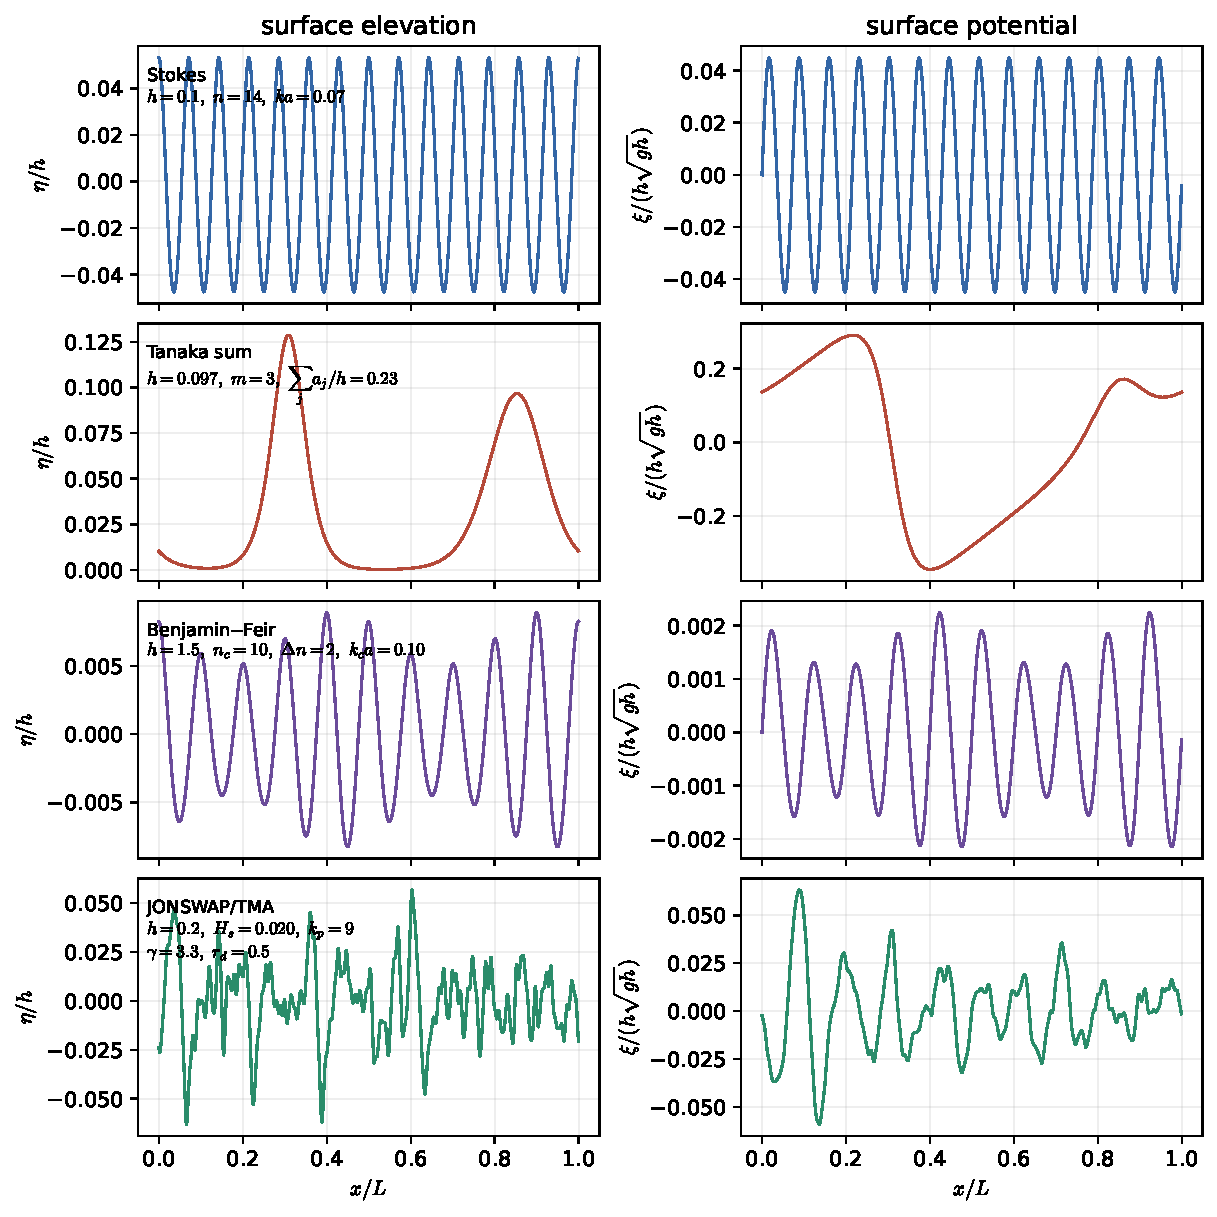
\includegraphics[width=\textwidth]
    {../figures/parameterized_corpus_case_examples.pdf}
  \caption{One constructed initial condition from each family.  The left
  column shows \(\eta/h\), and the right column shows
  \(\xi/(h\sqrt{gh})\), with \(g=1\).  These are
  examples of the formulas above, not cases selected by model error.}
  \label{fig:family-examples}
\end{figure}
\FloatBarrier

\section{One reference rollout and one whole-trajectory decision}
\label{sec:rollout}

Stokes cases are static.  Tanaka, Benjamin--Feir, and random-sea cases are
evolved with the same order-six DNO.  Define the internal output
\[
  \Gint(\eta;h)\xi
  =
  \mathcal G_{6}^{1024,8}
    (P_{128}\eta;h)(P_{128}\xi).
\]
The discrete Zakharov equations used for the rollout are
\begin{align}
  \eta_t
  &=
  \Gref(\eta;h)\xi, \notag\\
  \xi_t
  &=
  P_{128}^{\circ}\!\left[
    -\eta-\frac12\xi_x^2
    +\frac{
      \bigl(\Gint(\eta;h)\xi+\eta_x\xi_x\bigr)^2
    }{2(1+\eta_x^2)}
  \right].
  \label{eq:zakharov}
\end{align}
The Zakharov surface formulation and the Craig--Sulem expansion follow the
formulation used by Xu and Guyenne~\cite{xu2009}.  The truncation order,
spatial grid, padding factor, and delivered Fourier band in this note are
fixed project choices.
The Craig--Sulem calculation inside $\Gint$ uses padding factor eight.  The
products written explicitly in the second line of \eqref{eq:zakharov} are
formed on a separate two-times Fourier grid before projection.

The linear gravity-wave part of \eqref{eq:zakharov} is advanced exactly in
Fourier space.  More precisely, write the right-hand side as
$L_hz+R_h(z)$, where $z=(\eta,\xi)$, $L_h$ is the linear part, and $R_h$ is
the remainder.  The change of variable
$v(t)=e^{-tL_h}z(t)$ gives
\[
  v_t=e^{-tL_h}R_h(e^{tL_h}v).
\]
The program applies the two-stage, fourth-order Gauss--Legendre method
(GL2) to this transformed equation.  This is the integrating-factor GL2
method described by Xu and Guyenne~\cite{xu2009}.  The step, iteration cap,
and residual test below are our fixed implementation settings.

The GL2 step is $0.01$.  At each step it solves two coupled internal stage
equations by at most four fixed-point updates.  For each stage and each
field separately, the remaining stage-equation mismatch is divided by the
larger of the stage norm, the fixed-point-map norm, and the smallest normal
floating-point number.  The largest of these relative mismatches must be at
most $10^{-8}$.  After a completed step the two state fields are projected
back to their prescribed Fourier bands.  A candidate state is stored every
$0.08$, exactly every eight steps; there is no time interpolation.
The step \(0.01\) was selected before production on a fixed 12-case panel.
All ten cases that completed at both steps \(0.01\) and \(0.005\) agreed to
at most \(1.126337\times10^{-5}\); the other two became incomplete under
both steps.  The \(0.005\) calculation is therefore a method-level check, not
a second rollout applied to each production case.

Tanaka and Benjamin--Feir request $0\leq t\leq200$.  A random sea uses the
peak period
\[
  T_p=\frac{2\pi}{\omega_p}
\]
and requests the last $0.08$-grid time no later than $16T_p$.  Cases with
different random-sea horizons may share a numerical batch, but each one is
judged only on its own requested prefix.

Suppose the initial condition already obeys its family's parameter rules.
There is then one trajectory decision:
\begin{equation}
  \boxed{\text{accept}
    \quad\Longleftrightarrow\quad
    \text{the fixed method returns one complete admissible trajectory}.}
  \label{eq:trajectory-acceptance}
\end{equation}
Here \emph{complete admissible trajectory} means that the calculation reaches
its requested final time, every GL2 stage has finite relative residual at
most \(10^{-8}\), every stage and updated state is finite, all saved
\(\eta\), \(\xi\), and \(\Gref(\eta;h)\xi\) values are finite, and
\[
  h+\eta(x_\ell,t_j)>0
\]
at every saved time \(t_j\) and grid point \(x_\ell\).  The final inequality
is the elementary geometric requirement that the graph of the free surface
remain above the flat bottom \(y=-h\).  It has already been checked at
\(t=0\) while assembling the initial batch and is checked again on every
saved state.  The recorded diagnostics state which clause failed; they are
not additional fitted filters.  A failed trajectory
contributes zero rows.  Keeping its finite prefix would systematically give
difficult cases only their earlier, easier states.

Only the one $\Delta t=0.01$ trajectory is run for each production case.
Sign changes, slope, extrema, spectrum, Hamiltonian drift, absolute target
size, visual appearance, and model error do not decide acceptance.

A static Stokes state has no trajectory.  It is kept only when its sampled
parameters obey the Stokes rules, its state and common target are finite, and
$h+\eta_0>0$ at every grid point.

\subsection{Endpoint diagnostics that do not reject cases}
\label{sec:endpoint-diagnostics}

Spatial roughness and sign changes remain useful for finding cases that merit
inspection, even though neither quantity decides acceptance.  We applied two
such rankings to the fixed method-level rollout panel.  We first removed the
two trajectories that did not reach their requested terminal time, exactly as
the corpus rule requires.  For the figures below, we then omit the three
JONSWAP/TMA cases because their intentionally broadband spectra otherwise
dominate both rankings and obscure comparison among the coherent-wave
families.  This second omission is only a presentation choice; it does not
remove any case from the corpus.  The displayed rankings therefore use five
completed Tanaka and Benjamin--Feir endpoints.  No last-finite frame from an
incomplete trajectory participates.

Let $\widehat\eta_k$ be the Fourier coefficients of an endpoint elevation
after removal of its mean.  Define its root-mean-square wavenumber by
\begin{equation}
  k_{\mathrm{eff}}(\eta)
  =
  \left(
    \frac{\sum_{k\ne0}k^2|\widehat\eta_k|^2}
         {\sum_{k\ne0}|\widehat\eta_k|^2}
  \right)^{1/2}.
  \label{eq:effective-wavenumber}
\end{equation}
This is large when a substantial fraction of the elevation energy lies at
short spatial scales; by convention it is zero when the denominator
vanishes.  Figure~\ref{fig:terminal-roughness} shows all five completed
non-JONSWAP/TMA cases in decreasing order.

\begin{figure}[ht]
  \centering
  \includegraphics[width=\textwidth]{../../outputs/paper_corpus_terminal_diagnostics_20260726/top_non_jonswap_terminal_spatial_roughness.pdf}
  \caption{Cases with the largest endpoint value of
  $k_{\mathrm{eff}}(\eta)$.  In each row, the dashed gray curve is the initial
  field, the colored curve is the terminal field, and the right panel shows
  the corresponding normalized Fourier amplitudes.  Every displayed
  trajectory completed its requested interval, and JONSWAP/TMA cases are
  omitted from this display.  The narrow Tanaka case has the largest value,
  $k_{\mathrm{eff}}=37.52$; spatial roughness alone is therefore not evidence
  of numerical failure.}
  \label{fig:terminal-roughness}
\end{figure}

For the second ranking, let
$f_\ell=[\Gref(\eta;h)\xi](x_\ell)$ at the endpoint and form the cyclic
forward differences
\[
  d_\ell=f_{\ell+1}-f_\ell,\qquad
  \ell=0,\ldots,1023,\qquad f_{1024}=f_0.
\]
Set $\tau=0.03\max_\ell|d_\ell|$, discard differences with
$|d_\ell|\leq\tau$, and count cyclic transitions between the signs of the
remaining differences.  Denote this count by
$C_{0.03}(\Gref(\eta;h)\xi)$.  The dead zone prevents roundoff-sized
differences from creating sign changes.  Figure~\ref{fig:terminal-signs}
shows all five completed non-JONSWAP/TMA cases.

\begin{figure}[ht]
  \centering
  \includegraphics[width=\textwidth]{../../outputs/paper_corpus_terminal_diagnostics_20260726/top_non_jonswap_terminal_sign_changes.pdf}
  \caption{Cases with the largest endpoint sign-change count in the cyclic
  forward difference of $\Gref(\eta;h)\xi$, after incomplete trajectories
  and the broadband JONSWAP/TMA display cases have been removed.  The
  completed Tanaka upper-corner and Benjamin--Feir upper-boundary cases lead
  with 48 and 40 changes, followed by the narrow Tanaka case with 18.  The
  count detects small oscillatory contributions but does not by itself show
  that a completed trajectory is numerically unstable, so it is retained only
  as a diagnostic.}
  \label{fig:terminal-signs}
\end{figure}
\FloatBarrier

\section{Selecting times after acceptance}
\label{sec:time-selection}

Time selection reduces storage; it never decides whether a case is accepted
and it never uses model error.  Stokes retains only $t=0$.
Tanaka and Benjamin--Feir have 2501 candidate times
\[
  t_j=0.08j,\qquad j=0,\ldots,2500,
\]
and retain exactly 200 distinct times, including both endpoints.

For Tanaka, define the total surface-slope energy
\[
  S_{\mathrm T,j}
  =
  \sum_{\ell=0}^{1023}
  |\eta_x(x_\ell,t_j)|^2
\]
and its discrete time difference
\[
  D S_{\mathrm T,j}
  =
  \begin{cases}
    S_{\mathrm T,1}-S_{\mathrm T,0},&j=0,\\
    (S_{\mathrm T,j+1}-S_{\mathrm T,j-1})/2,&1\leq j\leq2499,\\
    S_{\mathrm T,2500}-S_{\mathrm T,2499},&j=2500.
  \end{cases}
\]
The Tanaka activity is
\[
  A_{\mathrm T,j}
  =
  \frac{|D S_{\mathrm T,j}|}
       {S_{\mathrm T,j}+10^{-12}}.
\]
Thus extra weight is given to times when the
surface shape changes rapidly.

For Benjamin--Feir, define
\[
  S_{\mathrm B,j}
  =
  \max_{0\leq\ell<1024}|\eta(x_\ell,t_j)|,
  \qquad
  A_{\mathrm B,j}
  =
  \left(
    S_{\mathrm B,j}
    -\min_{0\leq r\leq2500}S_{\mathrm B,r}
  \right)^4.
\]
This emphasizes large surface-elevation excursions; it is the maximum
absolute elevation, not an analytic-signal envelope.

Let $F=\mathrm T$ denote Tanaka and $F=\mathrm B$ denote Benjamin--Feir.
Each activity sequence $A_{F,j}$ is smoothed by a fixed Gaussian in the time
index.  Its standard deviation is 50 candidate times for Tanaka and 20 for
Benjamin--Feir.  The kernel stops at three standard deviations, and values
beyond either endpoint are replaced by that endpoint value.  If
$\widetilde A_{F,j}$ is the smoothed activity, the selection weights are
\[
  p_{F,j}
  =
  \frac{1-\alpha_F}{2501}
  +
  \alpha_F
  \frac{\widetilde A_{F,j}}
       {\sum_{r=0}^{2500}\widetilde A_{F,r}},
  \qquad
  \alpha_F=
  \begin{cases}
    0.50,&\text{Tanaka},\\
    0.85,&\text{Benjamin--Feir}.
  \end{cases}
\]
If all activities vanish, the second term is replaced by a uniform weight.
The program takes fixed midpoint quantiles of the cumulative weights, pins
the first and last times, and clips each quantile index so that enough unused
indices remain for all later quantiles.  A forward pass then advances any
repeated index to the next unused one.  The result is deterministic.

For a random sea, let
\[
  T_s=0.08\left\lfloor\frac{16T_p}{0.08}\right\rfloor,
  \qquad J_s=T_s/0.08.
\]
It retains the 16 indices
\[
  j_\ell=
  \left\lfloor\frac{\ell J_s}{15}+\frac12\right\rfloor,
  \qquad \ell=0,\ldots,15.
\]
These are approximately uniform and include $0$ and $T_s$.

\section{Identity, splitting, quotas, and storage}
\label{sec:records}

\subsection{Case identity and data splits}

The full case identity consists of
\[
  (\text{family},\ \text{revision},\ \text{split},\
    \text{stream},\ \text{attempt}).
\]
Its deterministic random stream instead uses these five integer seed words:
\[
  (\text{split root},\ \text{family},\ \text{revision},\
    \text{stream},\ \text{attempt}).
\]
These words seed NumPy's PCG64 generator.  The split roots are
\[
  \begin{array}{c|ccc}
    \text{split}&\text{training}&\text{validation}&\text{test}\\ \hline
    \text{root}&2026072210&2026072204&2026072205.
  \end{array}
\]
The split, parameter category, and entire sampled specification are written
before construction or integration.  A rejection remains attached to that
split.  All stored times from one trajectory therefore stay together, so
nearby times from the same numerical solution cannot cross into validation
or test.

\subsection{Accepted-case quotas}

A quota is a required number of accepted complete cases, not a number of
attempts or stored rows.  Suppose a family has $m$ ordered parameter
categories and requires $C$ accepted cases.  Write
\[
  C=bm+r,\qquad 0\leq r<m.
\]
The first $r$ categories receive $b+1$ cases and the other categories receive $b$.
This is the most even integer division possible.

A failed attempt is replaced only in its original category.  A category assigned
$Q$ accepted cases may use at most $4Q$ recorded attempts.  If the
resolved attempts reach this bound without filling $Q$, the family run stops
as incomplete.  Another category cannot fill the deficit.  The factor four
only bounds computation; it does not change any case-level decision.  The
Stokes amplitude redraws described above are internal to one attempt.

\subsection{Files and combined view}

An accepted row stores three length-1024 spatial arrays
$\eta$, $\xi$, and $\Gref(\eta;h)\xi$ in float32, together with float64 depth
and time, its selected candidate-time index, and its case-local index in that
array file.
The case record preserves the sampled parameters and numerical decision for
both accepted and rejected attempts.  It also binds the family, split,
random stream, numerical settings, software versions, source hashes, and
array checksum.

After the four families have been generated for all three splits, the
combined builder checks the records, shapes, checksums, numerical settings,
and required counts.  It then writes a compact row-to-case index pointing to
the existing arrays rather than copying them.  This index is the dataset
view read by the trainer.

\section{Production size and trainer handoff}
\label{sec:handoff}

The first checkpoint requests, from \emph{each} family,
\[
  2048\ \text{training},\qquad
  1024\ \text{validation},\qquad
  1024\ \text{test cases}.
\]
The four families therefore contain 16,384 accepted cases in total.
For one accepted case from each family, the stored-row count is
\[
  1+200+200+16=417.
\]
The exact split counts are
\begin{table}[ht]
  \centering
  \small
  \begin{tabular}{lrr}
    \toprule
    Split & Accepted cases & Stored rows\\
    \midrule
    Training & 8,192 & 854,016\\
    Validation & 4,096 & 427,008\\
    Test & 4,096 & 427,008\\
    \midrule
    Total & 16,384 & 1,708,032\\
    \bottomrule
  \end{tabular}
\end{table}
The current uncompressed estimate for the field archives and row map is
19.62 GiB.
Training then grows by additive, disjoint chunks to
\[
 C_{\mathrm{tr}}\in\{2048,4096,8192,16384\}
\]
accepted cases per family; validation and test remain fixed at 1024 cases per
family.  The resulting cumulative sizes are
\begin{center}
\begin{tabular}{rr}
  \toprule
  Training cases per family & Total stored rows \\
  \midrule
  2,048  & 1,708,032 \\
  4,096  & 2,562,048 \\
  8,192  & 4,270,080 \\
  16,384 & 7,686,144 \\
  \bottomrule
\end{tabular}
\end{center}
Thus 2048 is a checkpoint, not the completed corpus.  The target at 16,384
contains 73,728 accepted cases across the four families and three splits.
Its 7,686,144 rows are close to the 7,633,989 rows in historical v9: 52,155
more rows, or 0.68\%.

Normalization is computed from all stored \emph{training} rows and from no
validation, test, or diagnostic rows.  Let $\eta_i$, $\xi_i$, and $h_i$
denote the elevation, potential, and depth in training row $i$, and let
$G_i^\star=\Gref(\eta_i;h_i)\xi_i$ denote its reference label.  Define
\[
  s_\eta=\max_{i,x}|\eta_i(x)|,\qquad
  s_\xi=\max_{i,x}|\xi_i(x)|,\qquad
  s_G=\max_{i,x}|G_i^\star(x)|.
\]
The intended corpus gives positive values for all three scales, and the
release audit verifies this before training.  The current loader uses one as
a defensive fallback if a nonpositive scale reaches it; that fallback is not
treated as validation of a malformed corpus.  The cached values are tied to
the checked dataset identity.
The trainer receives
\[
  \eta/s_\eta,\qquad
  \xi/s_\xi,\qquad
  \log(h/h_\star),\qquad
  \Gref(\eta;h)\xi/s_G,
\]
where the reference length is $h_\star=L/(2\pi)=1$ on the production domain.
The paper-corpus training command must explicitly select this scale
normalization with \texttt{--norm scale}; the trainer's generic min--max
default is not the rule stated here.

At every training epoch, the loader chooses one stored time uniformly from
every accepted training case.  Thus each family contributes
$C_{\mathrm{tr}}$ samples per epoch even though the archive stores different
numbers of times per case.  Validation uses one fixed deterministic time per
case.  Airy,
manufactured-DNO, and sparse-Fourier states remain diagnostic tests and do
not enter training or its normalization.

\section{Checks before bulk generation}
\label{sec:release}

Grid, truncation, padding, spectral window, and time step are chosen on
fixed method-level panels before bulk generation.  They are not re-estimated
for individual production cases.  The final execution check asks for one
accepted case, using all production settings and the present
single-trajectory executor, from every trajectory parameter category:
\[
  11\ \text{Tanaka}
  +66\ \text{Benjamin--Feir}
  +27\ \text{JONSWAP/TMA}
  =104\ \text{categories}.
\]
This \emph{104-category pilot} uses the production solver, trial batch size four,
and at most four attempts per category.  It is kept separate from the final
corpus.  The four static Stokes categories have already passed their exact
calculation under generator revision 2: all four cases were accepted and all
four quality-decision masks were zero.  The pilot asks whether every declared
trajectory category can be
constructed and evolved; one case per category does not estimate a population
rejection rate.

Bulk generation begins only after this pilot completes, its wall time and
peak memory are recorded, and its result determines the production batch
size.  The final audit checks exact case and row counts, disjoint splits,
finite stored arrays, positive depths, zero-row failed cases, checksums, and
training-only normalization.

\paragraph{Present status.}
As of 27 July 2026, exact generator-revision-2 calculations have passed for
the four static Stokes categories, and the 104-category trajectory pilot is
running.  Bulk generation remains conditional on that pilot passing.
Therefore the current single-trajectory contract is not yet validated across
all trajectory parameter categories; the 7,686,144-row target corpus has not
been generated; its population acceptance rates and runtime are unknown; and
no reported model has been trained on it.  This note is the frozen
construction contract, not a report of a completed replacement dataset.

{\footnotesize
\begin{thebibliography}{99}
\setlength{\itemsep}{0pt}

\bibitem{fenton1985}
J.~D. Fenton,
\newblock A fifth-order Stokes theory for steady waves,
\newblock \emph{Journal of Waterway, Port, Coastal, and Ocean Engineering}
111(2) (1985), 216--234.

\bibitem{zhao2024}
K.~Zhao, Y.~Wang, and P.~L.-F. Liu,
\newblock A guide for selecting periodic water wave theories,
\newblock \emph{Coastal Engineering} 188 (2024), 104432.

\bibitem{xu2009}
L.~Xu and P.~Guyenne,
\newblock Numerical simulation of three-dimensional nonlinear water waves,
\newblock \emph{Journal of Computational Physics} 228 (2009), 8446--8466,
\newblock doi:10.1016/j.jcp.2009.08.015.

\bibitem{tanaka1986}
M.~Tanaka,
\newblock The stability of solitary waves,
\newblock \emph{Physics of Fluids} 29(3) (1986), 650--655,
\newblock doi:10.1063/1.865459.

\bibitem{benjaminfeir1967}
T.~B. Benjamin and J.~E. Feir,
\newblock The disintegration of wave trains on deep water. Part 1. Theory,
\newblock \emph{Journal of Fluid Mechanics} 27(3) (1967), 417--430,
\newblock doi:10.1017/S002211206700045X.

\bibitem{dommermuth1987}
D.~G. Dommermuth and D.~K.~P. Yue,
\newblock A high-order spectral method for the study of nonlinear gravity
waves,
\newblock \emph{Journal of Fluid Mechanics} 184 (1987), 267--288,
\newblock doi:10.1017/S002211208700288X.

\bibitem{hasselmann1973}
K.~Hasselmann et al.,
\newblock Measurements of wind-wave growth and swell decay during the Joint
North Sea Wave Project (JONSWAP),
\newblock \emph{Erg\"anzungsheft zur Deutschen Hydrographischen Zeitschrift},
Reihe A(8), No.~12, 1973.

\bibitem{bouws1985}
E.~Bouws, H.~G\"unther, W.~Rosenthal, and C.~L. Vincent,
\newblock Similarity of the wind wave spectrum in finite depth water:
1. Spectral form,
\newblock \emph{Journal of Geophysical Research: Oceans} 90(C1) (1985),
975--986,
\newblock doi:10.1029/JC090iC01p00975.

\end{thebibliography}
}

\end{document}
